%
% To make graphic on linux....(require ImageMagic installed)
%
% pdflatex thisfile.tex
% convert -density 300 thisfile.pdf -resize 640x480 thatfile.png 
%
% On Windows 10.... copy ImageMagic's convert.exe to your path 
% or rename it imgconvert.exe
% Get recent version of GhostScript
%
% pdflatex thisfile.tex
% convert -density 300 thisfile.pdf -resize 640x480 thatfile.png 
%
% Trouble? See this thread
%
% https://tex.stackexchange.com/questions/11866/compile-a-latex-document-into-a-png-image-thats-as-short-as-possible/11880#11880
%
\documentclass{standalone}
\usepackage{tikz}

\author{CC-BY-2016 James B. Wilson}
\date{2016}
\date{today}
\begin{document}
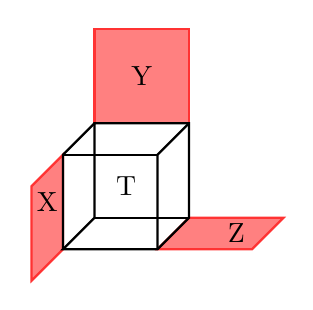
\begin{tikzpicture}[scale=.2]
\%
\fill[color=red!50] (-2,0) -- (-2,6) -- (-4,4) -- (-4,-2) -- (-2,0);
\draw[thick, color=red!80] (-2,0) -- (-2,6) -- (-4,4) -- (-4,-2) -- (-2,0);
\node at (-3,3) {X};
%
\fill[color=red!50] (0,8) -- (6,8) -- (6,14) -- (0,14) -- (0,8);
\draw[thick, color=red!80] (0,8) -- (6,8) -- (6,14) -- (0,14) -- (0,8);
\node at (3,11) {Y};
%
\fill[color=red!50] (6,2) -- (12,2) -- (10,0) -- (4,0) -- (6,2);
\draw[thick, color=red!80] (6,2) -- (12,2) -- (10,0) -- (4,0) -- (6,2);
\node at (9,1) {Z};
%
\draw[thick] (0,2) -- (0,8) -- (6,8) -- (6,2) -- (4,0) -- (-2,0) -- (0,2);
\draw[thick] (-2,0) -- (-2,6) -- (0,8);
\draw[thick] (4,0) -- (4,6) -- (6,8);
\draw[thick] (-2,6) -- (4,6);
\draw[thick] (0,2) -- (6,2);
\node at (2,4) {T};
\end{tikzpicture}
\end{document}
